\documentclass[a4paper, 12pt]{article}

\usepackage[no-math]{fontspec-xetex}
\setmainfont{IBM Plex Sans}
\usepackage[english, russian]{babel}

\usepackage{blindtext}
\usepackage{microtype}
\usepackage{geometry}

\usepackage{amsmath, amsfonts, amssymb, amsthm, mathtools}
\usepackage{MnSymbol}
\usepackage{physics}

\usepackage{graphicx, wrapfig, caption, subcaption}
\usepackage{color, xcolor}

\usepackage{titlesec}
\usepackage[document]{ragged2e}
\usepackage{enumitem}
\usepackage{hyperref}
\usepackage{import}
%\usepackage{csvsimple}
%\usepackage[none]{hyphenat}
%\usepackage{mathastext}

\graphicspath{{figures/}}
\geometry{margin=6em}
\geometry{bottom=6em}

% Настройки заголовков
\titleformat{\section}[hang]{\Large}{}{0em}{}{}
\titleformat{\subsection}[hang]{\large}{}{0em}{}{}

% Это предотвратит разрыв слов
\hyphenpenalty=10000
\exhyphenpenalty=10000

% Настройки параграфов текста
\setlength{\parindent}{0em}
\setlength{\parskip}{1em}
\renewcommand{\baselinestretch}{1.1}

% Настройки списков
\setlist{leftmargin=*, noitemsep}

% Настройки таблиц
\setlength{\tabcolsep}{2em}
\renewcommand{\arraystretch}{1.3}

% Настройки ссылок
\hypersetup{colorlinks=true, linkcolor=blue, urlcolor=blue}

\title{Определение коэффициента вязкости глицерина}
\author{Роман Ухоботов, Николай Грузинов}
\date{}%собрано \today}

\begin{document}
    \maketitle


    \section{Цель работы}\label{sec:target}
    Определить коэффициент вязкости жидкости (глицерина) при помощи исследования падающих в нем тел.


    \section{Используемое оборудование}\label{sec:tools}
    \begin{enumerate}
        \item Мерный цилиндр с глицерином
        \item Набор калиброванных шариков из стали и свинца
        \item Измерительные приборы --- весы, микрометр, линейка
        \item Оборудование для съёмки --- камера телефона и фонарь
    \end{enumerate}


    \section{Теория}\label{sec:theory}

    Для падения тел сферической формы в вязких жидкостях действует формула Стокса:
    \[F(v) = -6 \pi r \eta v\]

    Поэтому II закон Ньютона для шарика с установившейся скоростью выглядит следующим образом:
    \[m g = 6 \pi r \eta v + \rho g V\]

    Выразим из него вязкость глицерина:
    \[ \eta = \frac{m g - \rho g V}{6 \pi r v} \]

    Мгновенную скорость шариков мы сможем без проблем получить из видео, но нужно понять,
    как быстро она устанавливается (спойлер: очень быстро).
    Попробуем грубо это оценить.

    Так выглядит II закон Ньютона для шарика в произвольный момент падения, вертикальная ось направлена вверх:
    \[ ma = - 6 \pi \eta r v - \rho g \frac{\pi d^3}{6} + mg \]

    Решив дифференциальное уравнение относительно скорости, мы получаем:
    \[ \tau = \frac{m}{6\pi r\eta}\ln \frac{mg - \rho gV - 6\pi r\eta v_0}{mg - \rho gV - 6\pi r\eta v} \]

    Так по абсолютно любой скорости мы сможем узнать, когда падающий шарик её имеет.


    \section{Ожидания от наблюдений}

    Мы предполагаем, что установившаяся скорость шарика будет зависеть от параметров самого шарика,
    а вязкость глицерина будет одинаковой независимо от наблюдаемого шарика.


    \section{Методика измерений}

    Мы решили, что точнее всего получится проанализировать видео падающего шарика с помощью алгоритма,
    чтобы установить его скорость и, соответственно, вязкость жидкости.
    Проделаем эксперимент 10 раз, используя 3 стальных и 7 свинцовых шаров трёх разных размеров:

    \vspace{1.5em}
    \begin{tabular}{l l l}
        \bfseries Number & \bfseries Diameter (mm) & \bfseries Mass (g) \\ \hline
        1                & 3.972                   & 0.2570             \\ \hline
        2                & 3.974                   & 0.2575             \\ \hline
        3                & 3.964                   & 0.2556             \\ \hline
        4                & 2.181                   & 0.0834             \\ \hline
        5                & 2.430                   & 0.0929             \\ \hline
        6                & 2.984                   & 0.1705             \\ \hline
        7                & 3.003                   & 0.1584             \\ \hline
        8                & 4.042                   & 0.3882             \\ \hline
        9                & 4.013                   & 0.3824             \\ \hline
        10               & 4.098                   & 0.3864             \\ \hline
    \end{tabular}
    \vspace{1.5em}

    Далее поочерёдно бросаем шарики в глицерин, записывая всю картину на видео.
    Полученную из видео зависимость позиции шариков от времени мы выложили
    \href{https://github.com/phys-labs-at-hse/glycerine/tree/master/particular_balls}{здесь}.


    \section{Расчёт}

    Сначала давайте оценим сверху, как быстро устанавливается скорость.

    Роняли мы шарики с 5см, откуда $v_0 = \sqrt{2g\cdot0.05} \approx 1$м/с
    Возьмём из них самый лёгкий, с параметрами $m = 0.0834$ г, $r = 2.181$ мм
    Также допустим, что вязкость будет больше 1 Па$\cdot$с
    Плотность глицерина $\rho = 1261$ кг/м3
    Посчитаем время, которое понадобится скорости, чтобы приблизиться к установившейся с точностью хотя бы до 1\%

    Если подставить все приведённые значения в формулу из теории, мы получим $\tau \approx 0.02$ с.

    То есть не пройдёт и 0.02 секунд, как скорость шарика установится!
    Этот результат чрезвычайно мал, достаточно мал,
    чтобы считать скорость установившейся \textbf{с самого начала падения}, а значит и на всём протяжении падения тоже.
    Далее мгновенную скорость будем считать установившейся.


    \section{Анализ}

    Построим по данным шариков зависимость глубины падения от времени:

    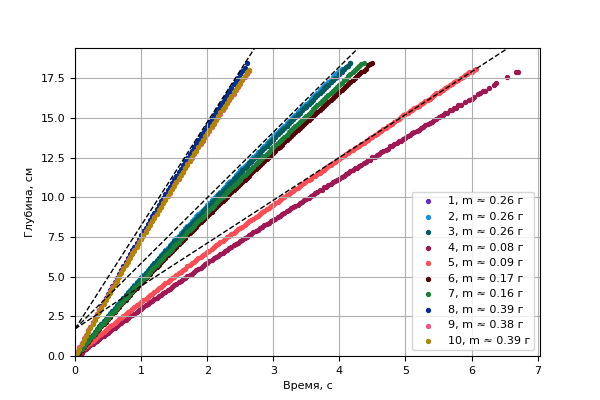
\includegraphics{position-time.png}

    На графике отчётливо видно разделение кривых на 3 группы: сверху зависимость,
    характерная большим свинцовым шарам (8-10), снизу малым свинцовым шарам (4-5),
    а средние свинцовые (6-7) и стальные шары (1-3) слились в одну группу посередине.

    Теперь, импользуя зависимости вязкости глицерина от скорости, выведенную в теории, построим график,
    отновываясь на мгновенной скорости шариков при данной глубине:

    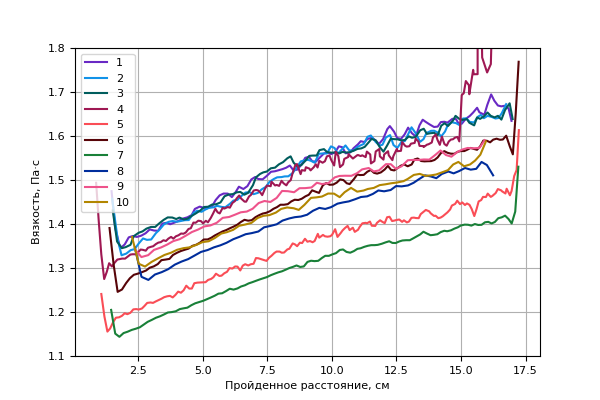
\includegraphics{viscosity-position.png}

\end{document}
